\documentclass[%
 reprint,
%superscriptaddress,
%groupedaddress,
%unsortedaddress,
%runinaddress,
%frontmatterverbose, 
%preprint,
%showpacs,preprintnumbers,
%nofootinbib,
%nobibnotes,
%bibnotes,
 amsmath,amssymb,
 aps,
%pra,
%prb,
%rmp,
%prstab,
%prstper,
%floatfix,
]{revtex4-1}

\usepackage{graphicx}   % for figures
\usepackage{epstopdf}
%\usepackage{epsfig}
%draft
\usepackage{dcolumn}
\usepackage{bm}	
\usepackage{amsmath}			
\usepackage{amsfonts}			
\usepackage{amssymb}			
\usepackage{latexsym}			
%\usepackage{floatrow}
\usepackage{color}
%\usepackage{thumbpdf}

\begin{document}

\title{Accounting for  beam-bending in classical ray tracing schemes for propagating realistic pulses in indirect drive ignition conditions}
\author{C. Ruyer}\email{charles.ruyer@cea.fr}
\affiliation{CEA, DAM, DIF, F-91297 Arpajon, France}
\affiliation{Universit\'e Paris-Saclay, CEA, LMCE, 91680 Bruy\`eres-le-Ch\^atel, France}
\author{A. Debayle}
\affiliation{CEA, DAM, DIF, F-91297 Arpajon, France}
\affiliation{Universit\'e Paris-Saclay, CEA, LMCE, 91680 Bruy\`eres-le-Ch\^atel, France}
\author{R. Riquier}
\affiliation{CEA, DAM, DIF, F-91297 Arpajon, France}
\author{P. Loiseau}
\affiliation{CEA, DAM, DIF, F-91297 Arpajon, France}
\affiliation{Universit\'e Paris-Saclay, CEA, LMCE, 91680 Bruy\`eres-le-Ch\^atel, France}
\author{P. E. Masson-Laborde}
\affiliation{CEA, DAM, DIF, F-91297 Arpajon, France}
\affiliation{Universit\'e Paris-Saclay, CEA, LMCE, 91680 Bruy\`eres-le-Ch\^atel, France}
\begin{abstract}
We propose a simple analytical modeling of the beam bending deviation of a spatially and temporally incoherent laser pulse in light of  hydrodynamic paraxial simulations and of interest for most high energy laser facilities.
A modified ray tracing scheme is then introduced and validated for accounting efficiently  for the centroid deviation in realistic conditions.
When applied to the propagation of the  inner cone in a full-scale simulation of a NIF experiment, a significant impact of the beam bending physics in two dimensions on the path of the laser is predicted, able to affect the refraction conditions on the gold hohlraume and possibly the capsule implosion symmetry.
\end{abstract}

\maketitle

\section{Introduction}
Many experiments conducted in multi-kilojoule laser facilities, whether the concern astrophysical phenomenon, high-energy-density physics \cite{Drake2006} or inertial confinement fusion \cite{Lindl_2004,He_2007,Cavailler_2005}, 
bring critical insights into  matter under extreme  conditions. 
In these facilities, the drive is used to heat  and compress the matter to millions of degrees and  Mega to Gigabar pressure. 
The predictability of these experiments  requires the precise understanding of the laser plasma interaction such as 
the mechanisms responsible of the energy deposition,  or   the growth of various instabilities such as stimulated Raman or Brillouin scattering  \cite{Shen_1965,Forslund_1973,POP_Liu_2009,hao_2013}, cross-beam energy transfer \cite{hao_2016}, two-plasmon decay  \cite{Dubois_1995,Russell_2001} or self-focusing  \cite{Wagner_1968}.

Furthermore, optical smoothing techniques as Random-Phase-Plates (RPP) or  spectral dispersion (SSD), often used in LMJ or NIF-class facilities, allow to reach a better control on the laser intensity profile \cite{Kato_1984,Skupski_1989}.
These techniques  degrade the spatial (RPP) and temporal coherence (SSD) of the  light,  resulting in intensity fluctuations on the scale of a few wavelength lasting a few picoseconds: the so-called speckles. 
They will in turn affect the plasma dynamics on macroscopic scales by affecting the energy deposition region  \cite[]{POP_Delamater_1996,Huser_2009}, the scattering direction  of the light wave \cite{Epstein_1986,PRL_Moody_96,POP_Debayle_2018,POP_Duluc_2019,Yin_2019,POP_Huller_2020} or the amount of expected reflectivity \cite[]{POP_Laffite_2010,PRL_Rousseaux_2016,POP_Masson_2016,Glize_2017,Winjum_2019}. Accounting for the hot-spot dynamics thus requires to capture the interplay between the micron or  sub-micron physics driving the   diffraction pattern of the RPP/SSD beam, with the millimeters and nanoseconds typical duration and size of the experiments. 
In this context, an hydrodynamical description of the plasma can be coupled with Maxwell equations \cite{Berger_1995,Still_2006,Loiseau_2006, Huller_2006}, however this formalism which fails to capture self-consistently Landau damping of acoustic waves may appear to be  too heavy numerically whenever  multi-dimensional effects,  solid-density physics or radiative phenomenons arise.

In such systems, we usually resort to a rough description of light \cite[]{POP_Zhang_2014,Lefebvre_2018},  such as the classical ray tracing scheme which, in its native form, only captures the wave refraction and basic energy deposition.
The proper description, by the ray tracing scheme,  of simple  light quantities  such as the intensity  of the wave or its local spectrum, is still an active area of research  \cite{Egorchenkov_2001, Colaitis_2014, Strozzi_2017}.
Although a large effort is made in improving these schemes by including back or side scattering of the light caused by wave mixing processes \cite[]{Strozzi_2017,POP_Debayle_2019},  
modeling the impact of plasma smoothing effects on the pulse propagation properties remains vastly unexplored \cite[]{POF_Anderson,POP_Still_2000,POP_Grech_2006,PRL_Grech_2009}.
 
Notably, this study  addresses the beam bending  of  a laser pulse \cite{PRL_Hinkel_1996,POP_Hinkel_1998,POP_Bezzerides_1998,POP_Rose_96,PRL_Montgomery} .
It occurs when the laser driven density fluctuations are advected by a flow, resulting,  due to a wave-guide effect, to the deflection of the electromagnetic wave off its original propagating axe. 
As this effect may take place in a perfectly homogeneous plasma, the beam deflection may adds up to the well-known refraction of light caused by density gradients. 
We will first briefly recall  the two and three dimensions modeling of Ref \cite[]{POP_Ruyer_2020}, which predict the deflection angle, in both the asymptotic and transient regime of a Gaussian laser pulse.
The model will then be extended to the centroid deviation of a spatially (using random phase plates) and temporally (with spectral dispersion) incoherent laser pulse in light of HERA paraxial simulations \cite{Loiseau_2006}.  
%n fluid-based codes such as HERA or PF3D  \cite{Berger_1995,Still_2006,Loiseau_2006, Huller_2006}. 
Our model  will then be included into 
a  ray-tracing description of the beam propagation, compared successfully to  hydrodynamic paraxial simulations. This will allow us to address the laser propagation in realistic indirect drive ICF plasma conditions, \emph{i.e.} inside an hohlraume and evidence a sensible impact of the beam bending on the light energy path. 
The last section gather our concluding remarks and perspectives. 

Finally, the SI unit system is used throughout this publication, dropping the Boltzmann constant (temperature in eV) and vectors are noted in bold symbols. 

\section{The beam bending of a spatio-temporally incoherent laser pulse}\label{sec:gauss}
\subsection{Speckle-scale Gaussian pulse beam bending}
%For simplicity, we will assume  subsequently, as in Ref. \cite[]{POP_Ruyer_2020},  that the electromagnetic waves are forward propagating only, thus excluding any back-scattering. 
In references \cite{POP_Rose_96,POP_Ruyer_2020}, proof is made that in the asymptotic regime (noted with a $\infty$ exponent) and in the small angle limit,  the transverse averaged Gaussian beam wavevector, $ \langle \mathbf{k}_\perp\rangle$ may be related to plasma parameters through,
 
  \begin{align}
\frac{1}{k_0} \frac{d \langle \mathbf{k}_\perp \rangle^\infty    }{d x} \cdot& \frac{ \mathbf{v}_d }{ \vert \mathbf{v}_d \vert } = \frac{d\theta^\infty}{dx}= - \frac{n_0 }{n_c}  \frac{  I_0 }{ 4 v_g n_c T_e } \sqrt{\frac{2}{\pi}}   \frac{\beta_\mathrm{k/f}^{(D)} }{ \sigma}     
  \, ,\label{eq:bbinf} \\
  \beta_\mathrm{k/f}^{(2)} &=  \Im\left[\alpha_\mathrm{k/f}\left(\frac{k_yv_d}{\vert k_y\vert}\right)\right] \frac{k_y}{\vert k_y\vert}  \, ,\label{eq:beta2} \\
  \beta_\mathrm{k/f}^{(3)} &=\frac{1}{2^{1/2}}\int_{0}^{\pi/2} d\theta \cos(\theta)\Im\left[ \alpha_{\mathrm{k/f}}\left( v_d \cos(\theta) \right)  \right]  \, ,\label{eq:beta3} 
\end{align}
where $D$ is the system dimension and  $\Im$ is the imaginary part of a complex. 
We introduced,  $k_0=2\pi/\lambda_0$, $n_0$, $n_c$ are the laser wave vector in vacuum, electron and laser critical density respectively, as well as  $\mathbf{v}_{d}$, $ m_{e/i}$, $T_{e/i}$, $v_g$, $I$, the plasma drift velocity (assumed to be the same for electrons and ions), electron/ion, mass, temperature, laser group velocity and intensity respectively. 
Moreover, either fluid ($f$ subscribe) or kinetic ($k$ subscribe), the above relations recover the same form with, 
\begin{align}
 \alpha_ \mathrm{k}    & = \frac{-\mathcal{Z}'( \zeta_e) }{2}\frac{\mathcal{Z}'( \zeta_i)   }{  \mathcal{Z}'( \zeta_i) +\mathcal{Z}'( \xi_e)\frac{ T_i }{  ZT_e} } \, ,\label{eq:drakek}
 \\
\zeta_{e/i} &=  \frac{-\mathbf{k}_\perp\cdot\mathbf{v}_{d} }{\vert \mathbf{k}_\perp \vert } \sqrt{ \frac{ m_{e/i} }{ 2T_{e/i} }  }   \label{eq:xi} \, , \\
 \alpha_f  & =\frac{\kappa}{1-\mathbf{M}_0^2\cos^2\theta +2i\gamma_0 \vert\mathbf{M}_0\vert \cos\theta}  \, .  \label{eq:drakeh} \\
 \cos(\theta)& = \frac{\mathbf{k}_\perp\cdot\mathbf{v}_{d} }{\vert \mathbf{k}_\perp \vert \vert \mathbf{v}_{d}\vert  } 
\end{align}
We also made use of the Mach number $\mathbf{M}_0= \mathbf{v}_d/c_s$ and of of $\mathcal{Z}'$, the first order derivative of the plasma dispersion function \cite{Fried_Gell-Mann_1960}.
 The normalized ion acoustic Landau damping rate verifies 
  \begin{align}
\gamma_0 &= \sqrt{\frac{2T_i }{m_ic_s^2 }} 
\Im\left[
\frac{  \mathcal{Z}'\left(x_i\right) 
+\frac{T_i}{Z_iT_e}  \mathcal{Z}'\left(x_e\right)   }{  \mathcal{Z}''\left(x_i\right) +\left(\frac{T_i}{Z_iT_e}\right)^{3/2}\sqrt{\frac{Z_im_e}{m_i}}  \mathcal{Z}''\left(x_e\right)    }
\right]\, , \nonumber \\
x_{e/i}&=\sqrt{\frac{m_{e/i}c_s^2}{2T_{e/i}}}\, .\label{eq:g0}
\end{align}
Choice has been made in this study to use the exact formula as the usual approximation [Eq. (10) in Ref. \cite{POP_Ruyer_2020}] yields an overestimation for some plasma parameters of interest subsequently.
For a Maxwellian plasma, the above equations show that   the beam bending rate remains independent of the drift velocity component parallel to the laser propagation, hence,  in the following,  we will assume  that $\mathbf{v}_e=\mathbf{v}_i=\mathbf{v}_d$ and is  transverse to the  $x$-axis.

The beam bending transient regime, as derived in 
 Ref. \cite[]{POP_Ruyer_2020}, \emph{i.e.} based on a fluid plasma response, does not depend on the dimension of the system. Hence, the temporal evolution of the deflection angle reads $d \theta/dx  =f(t)d \theta^{\infty}/dx $   where $f(t)$ tends toward unity in a few Landau damping times.
 
One can also include the thermal corrections of Ref. \cite[]{Bychenkov_2000} to account for non local thermal effects on the density fluctuation amplitude.
In that case,
\begin{align}
     \hat{\Phi}_k&= -A_k\frac{I(\mathbf{k}_\perp)}{2n_c T_e v_g} \, ,\nonumber\\
     A_k(u)   &= \frac{1}{2} +Z\left( \frac{0.074}{u^2}+ \frac{0.88}{u^{4/7}} + \frac{2.54}{1+5.5u^2} \right) \, ,\nonumber \\ 
     u &=\vert \mathbf{k}_\perp \vert\lambda_\mathrm{mfp} \sqrt{Z_i}\label{eq:nl}\, ,
\end{align}
where $\lambda_\mathrm{mfp}$ is the electron mean free path. 
Hence, the time-dependent Gaussian beam bending deflection rate with non-local corrections follows,
  \begin{align}
  \frac{d\theta }{dx}= - f(t) A_k \frac{n_0 }{n_c}  \frac{  I_0 }{ 4 v_g n_c T_e } \sqrt{\frac{2}{\pi}}   \frac{\beta_\mathrm{k/f}^{(D)} }{ \sigma}     
  \, .\label{eq:bbf} 
\end{align}

\begin{figure}
\begin{tabular}{c}
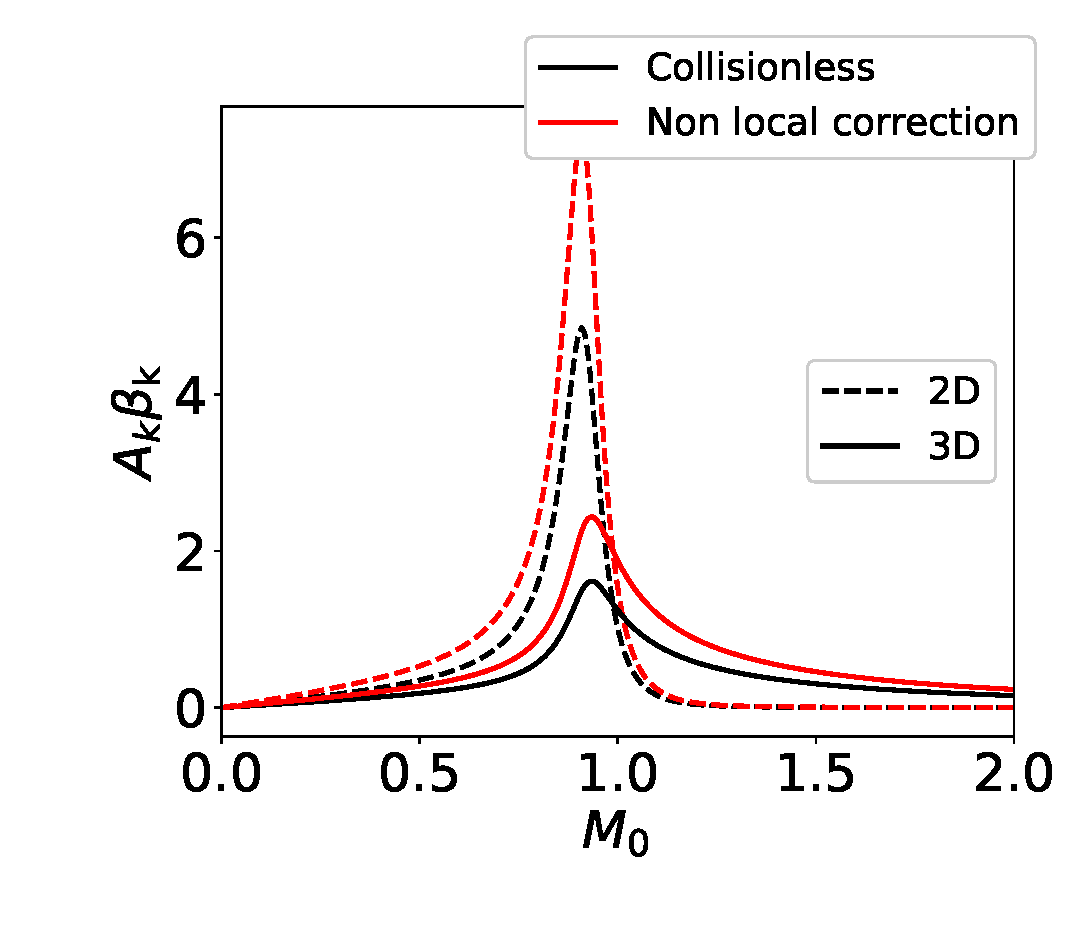
\includegraphics[scale=0.39]{Figure_1.eps}
\end{tabular}
\caption{ \label{fig:2d3dnl}
Product $A_k  \beta_\mathrm{k}^{(D)}$, as predicted by Eqs. \eqref{eq:beta2}-\eqref{eq:beta3} and \eqref{eq:nl},  for a He$^{2+}$ plasma  with $T_e=2\,\rm keV$, $Z_iT_e/T_i=3$ and $n_e=10^{21}\,\rm cm^{-3}$ and as a function of the Mach number.
The collisionless case in black lines corresponds to $A_k\equiv 1/2$.}
\end{figure}

Figure \ref{fig:2d3dnl} compares the value of  $\mathcal{A}  \beta_\mathrm{k}^{(D)}$ in two and three dimensions (dashed and plain lines respectively) for a collisionless plasma (for $\mathcal{A} \equiv1/2$ in black) and with the non-local correction of Eq. \eqref{eq:nl} (in red).  
The beam bending rate is more peaked around Mach numbers, $M_0=\vert v_d\vert /c_s$, close to unity for a planar geometry than in the  realistic case. Although the peaked value is roughly twice smaller for $D=3$ than for $D=2$,  it becomes larger in the realistic geometry when $M_0\gtrsim 1$.
Finally,  the thermal correction of Eq. \eqref{eq:nl} increases as expected the bending rate. For this choice of parameters ($T_e=2\,\rm keV$ and $n_e=10^{20}\,\rm cm^{-3}$), $A_k\simeq 0.75$ and should increase as the electron mean-free-path becomes shorter.

\subsection{Bending of a finite coherence-time speckle} \label{sec:speckle}
In light of our speckle-scale modeling, we propose to  quantify the effect on the laser deflection of
the broadening of the its temporal spectrum (SSD).
This technics, routinely used in multi-kilojoule class laser facilities, are  known to  qualitatively  reduce  the beam bending deflection   \cite{POP_Delamater_2000} by   causing the speckles to vanish and change position periodically \cite[]{phd-Duluc,POP_Duluc_2019}.
The ensuing finite speckle coherence time can be 
related to the modulator modulation period, $\omega_m$,  and  number of modes, $\Delta $,  through $\tau_\mathrm{SSD}=[(2\Delta+1)\omega_m]^{-1}$ \cite[]{Skupski_1989} and is usually of the order of a few picoseconds for $0.35\rm\mu m$-wavelength lasers. 
These time scales, much shorter than an acoustic Landau damping time $1/\nu \gtrsim 10\,\rm ps$, do not allow the beam bending to reach its asymptotic limit, thus yielding smaller deflection angles.


\begin{figure}
\begin{tabular}{c}
%(a) $\log_{10}[ \Delta \theta (\tau_\mathrm{SSD})]$\\
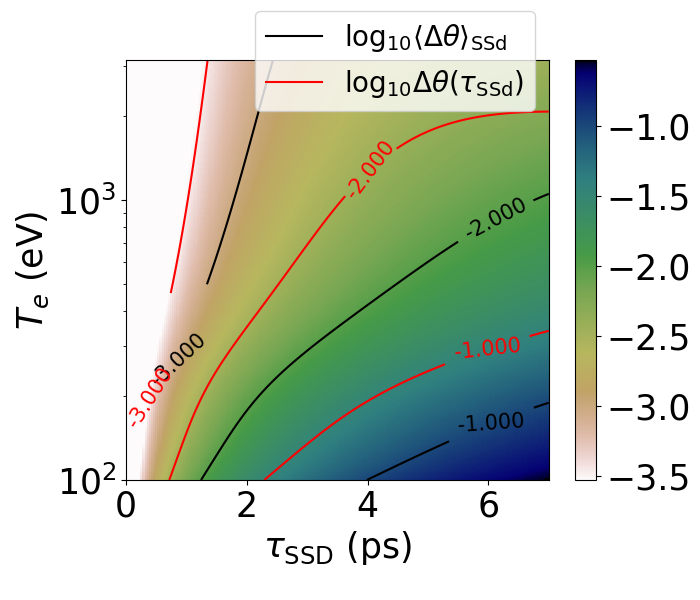
\includegraphics[scale=0.39]{paramssd.png}%\\
%(b) $\log_{10}[ \Delta \theta_\mathrm{SSD}]$\\
%\includegraphics[scale=0.39]{Dthmoy_15e14_2e-1nc_f8_3w.png}\\
\end{tabular}
\caption{ \label{fig:thssd}
Three dimensions deflection angle in  logarithmic scale  and  radiants, $\langle \Delta \theta \rangle_\mathrm{SSD}$ from Eq. \eqref{eq:dthssd} as a colormap and black contours and  $  \Delta \theta (\tau_\mathrm{SSD})$  as red contours using Eq. (31) of Ref. \cite{POP_Ruyer_2020}, \emph{i.e.} for a speckle of length $2\pi f_\sharp^22\pi/k_0$.  Use is made of the non local correction and the parameters are  $I_0=1.5\times 10^{15}\, ,\rm W.cm^{-2}$, $2\pi/k_0=0.35\,\rm\mu m$ and $f_\sharp=6.5$ in a He$^{2+}$ plasma  with $Z_iT_e/T_i=3$, $n_e=1.8\times 10^{21}\,\rm cm^{-3}$ and $M_0=0.9$.}
\end{figure}
We will mimic the effect of the SSD on the  resulting speckle scale beam bending rate  by assuming that the speckles disappear after a time $\tau_\mathrm{SSD}$. Hence the temporally averaged deflection angle is related to  Eq. \eqref{eq:bbf} through
\begin{equation}\label{eq:dthssd}
\langle \Delta \theta \rangle_\mathrm{SSD}=\frac{1}{\tau_\mathrm{SSD}}\int_0^{\tau_\mathrm{SSD}} \Delta \theta(t)dt\, .
\end{equation}
Figure \ref{fig:thssd} illustrates as a colormap and black contours for a moderately intense speckle (for  $2\pi/k_0=0.35\,\rm\mu m$,  $I_0=1.5\times 10^{15}\, ,\rm W.cm^{-2}$ and a focal number  $f_\sharp=6.5$, propagating in  a  He$^{2+}$ plasma with $n_e=0.2n_c$ and $M_0=0.9$),   the Gaussian pulse averaged   deflection  in logarithmic scale. As expected $\langle \Delta \theta \rangle_\mathrm{SSD}$ is maximized for large times and small temperature, reaching $\simeq 0.1$ (\emph{i.e.}, $100\, \rm \mu m$ per millimeter of propagation) at $(\tau_\mathrm{SSD}, T_e) \simeq (6 \, \mathrm{ps}, 200\,\mathrm{eV})$.
Moreover, a modest but not negligible, averaged deflection angle of $\sim 0.01$ (\emph{i.e.}, $10\, \rm \mu m$ per millimeter of propagation)  is also predicted for  
$(\tau_\mathrm{SSD}, T_e) \sim (6 \, \mathrm{ps}, 1\,\mathrm{keV})$.
Looking at the maximum deflection  in red contours, much larger values are reached such as $\Delta \theta(\tau_{\tau_\mathrm{SSD}})=0.1$  as soon as $(\tau_\mathrm{SSD}, T_e) \sim (6 \, \mathrm{ps}, 300\,\mathrm{eV})$ or $\Delta \theta(\tau_{\tau_\mathrm{SSD}})=0.01$   $  (6 \, \mathrm{ps}, 2\,\mathrm{keV})$, demonstrating a large scattering disparities over the speckles life-time. Hence, the  hot spot scale beam bending should result not only in a deviation of the laser  pulse centroid but also in the broadening of its  width. 

The beam bending that occurs during the propagation of a realistic laser pulse results from the superposition of the  various  speckles contributions. 
Although Fig. \ref{fig:thssd} illustrates the  bending of  a moderate intensity speckle,  predicting the amount of energy effectively deflected  requires to account for all the intensity fluctuations which form the realistic beam. 

%So as to capture the  bending rates of a SSD beam, we propose to average the deflection angle (using Eq. \eqref{eq:dtht}) over a   coherence time, giving
%\begin{align}
%\Delta \theta_\mathrm{SSD} &= %\frac{1}{\tau_\mathrm{SSD}}\int_0^{\tau_\mathrm{SSD}} \Delta %\theta(t)dt  \, ,\label{eq:dthssd}
%\end{align}
%When using the above deflection angle in our ray tracing model, we not only reduce the effect of SSD on the speckle dynamics  to a coherence time \cite{phd-Duluc}, but we also  choose to neglect  the first $\tau_\mathrm{SSD} $ of the bending dynamics.

\section{Hydrodynamic beam bending of a realistic pulse}

\subsection{Effect of temporal smoothing on the beam bending of a  $3\omega$-laser}\label{sec:parax}
\begin{figure*}
\begin{tabular}{ccc}
(a) H$^+$, $T_e=2\, \rm keV$,  $T_i=300\, \rm eV $ & (b) H$^+$, $T_e=1\, \rm keV$,  $T_i=100\, \rm eV $&(c) He$^{2+}$, $T_e=2\, \rm keV$, $T_i=500\, \rm eV $\\
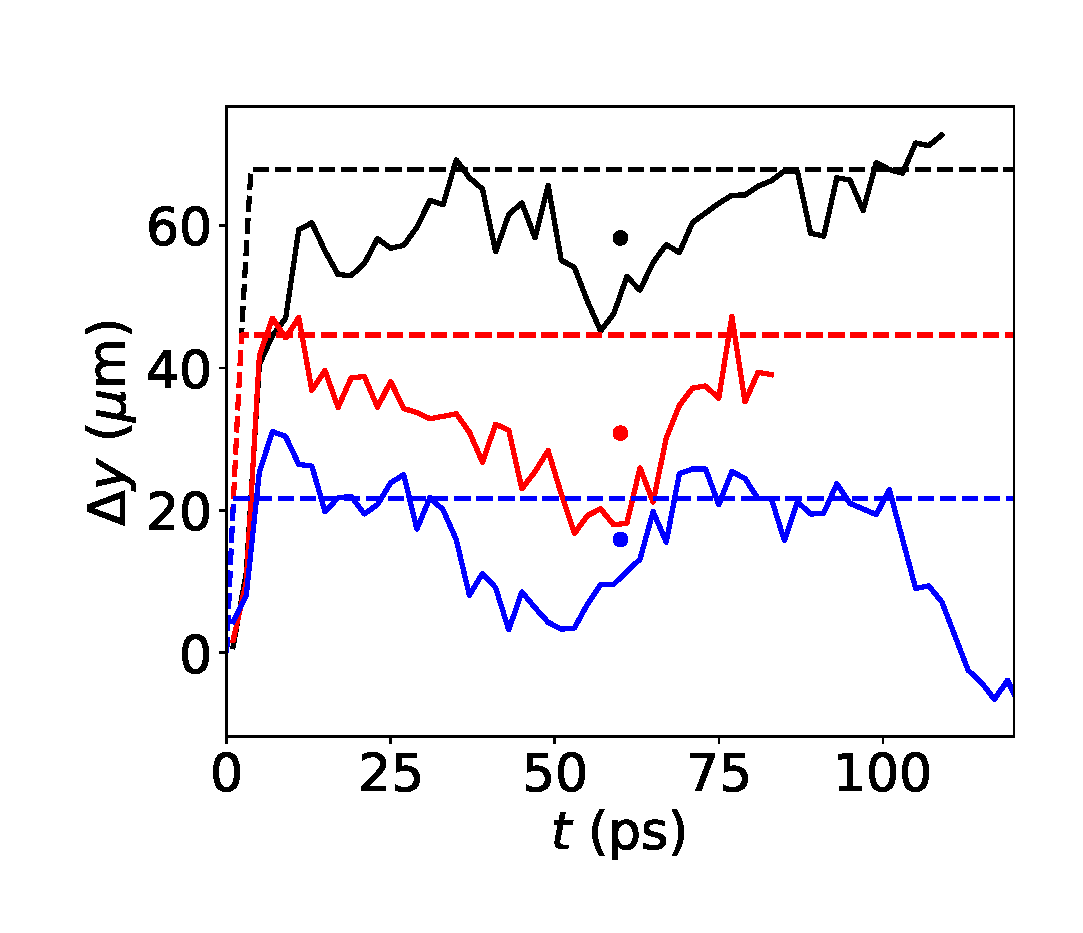
\includegraphics[scale=0.32]{bbssd_H300.eps}&
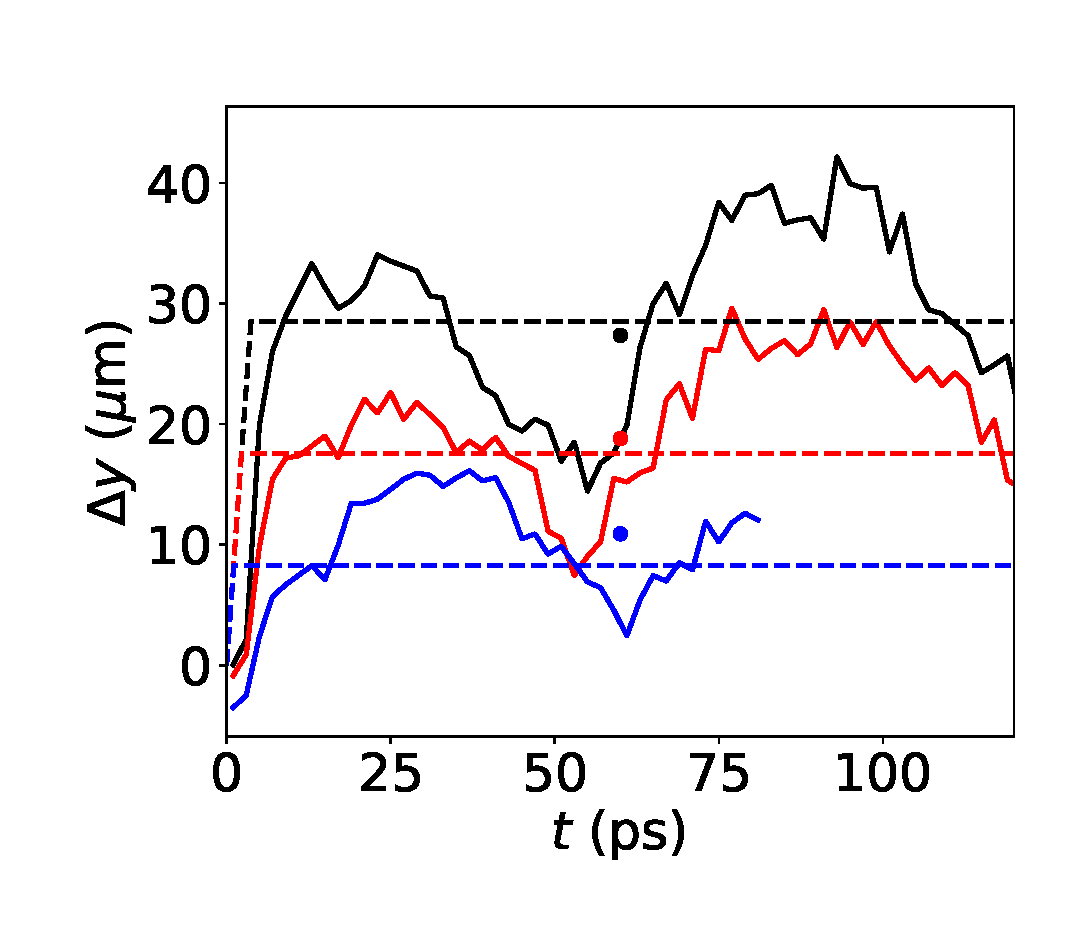
\includegraphics[scale=0.32]{bbssd_H100.eps}&
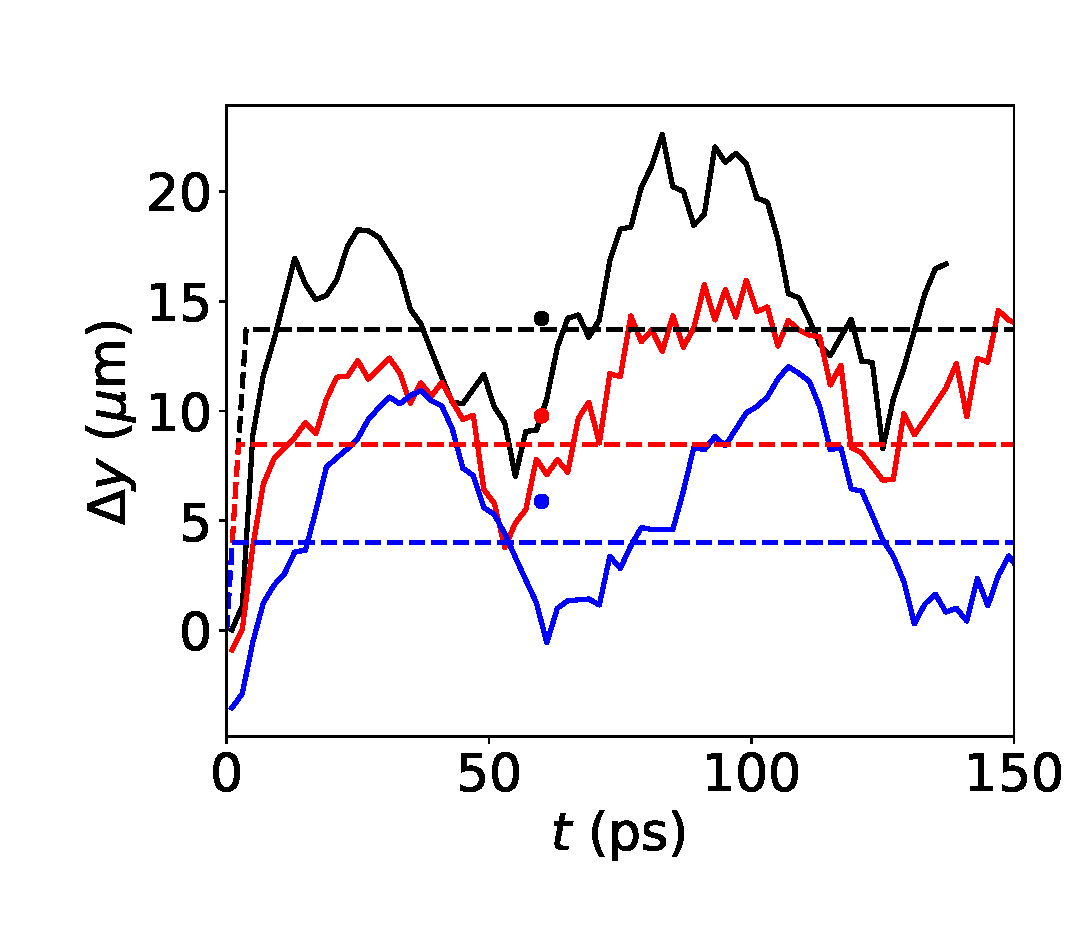
\includegraphics[scale=0.32]{bbssd_He.eps}\\
(d)&(e)&(f)\\
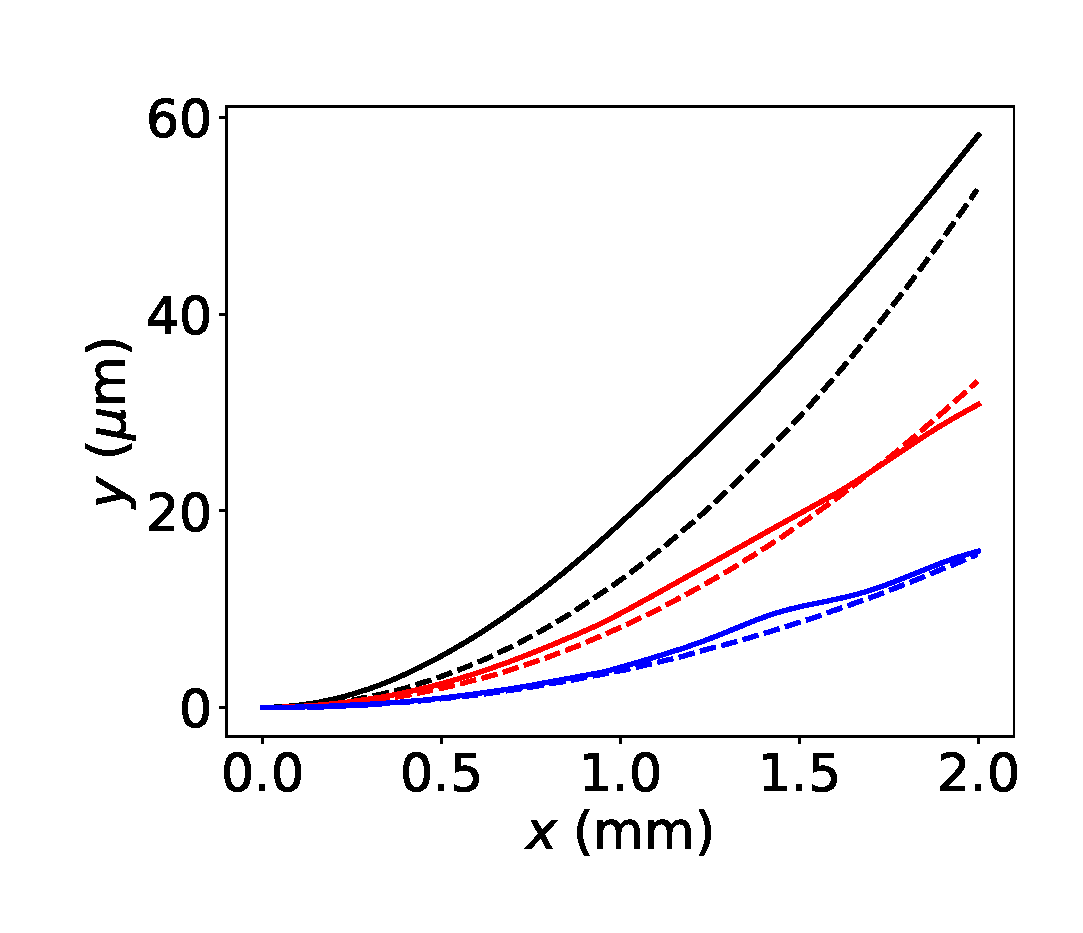
\includegraphics[scale=0.32]{rayparaxH300.eps}&
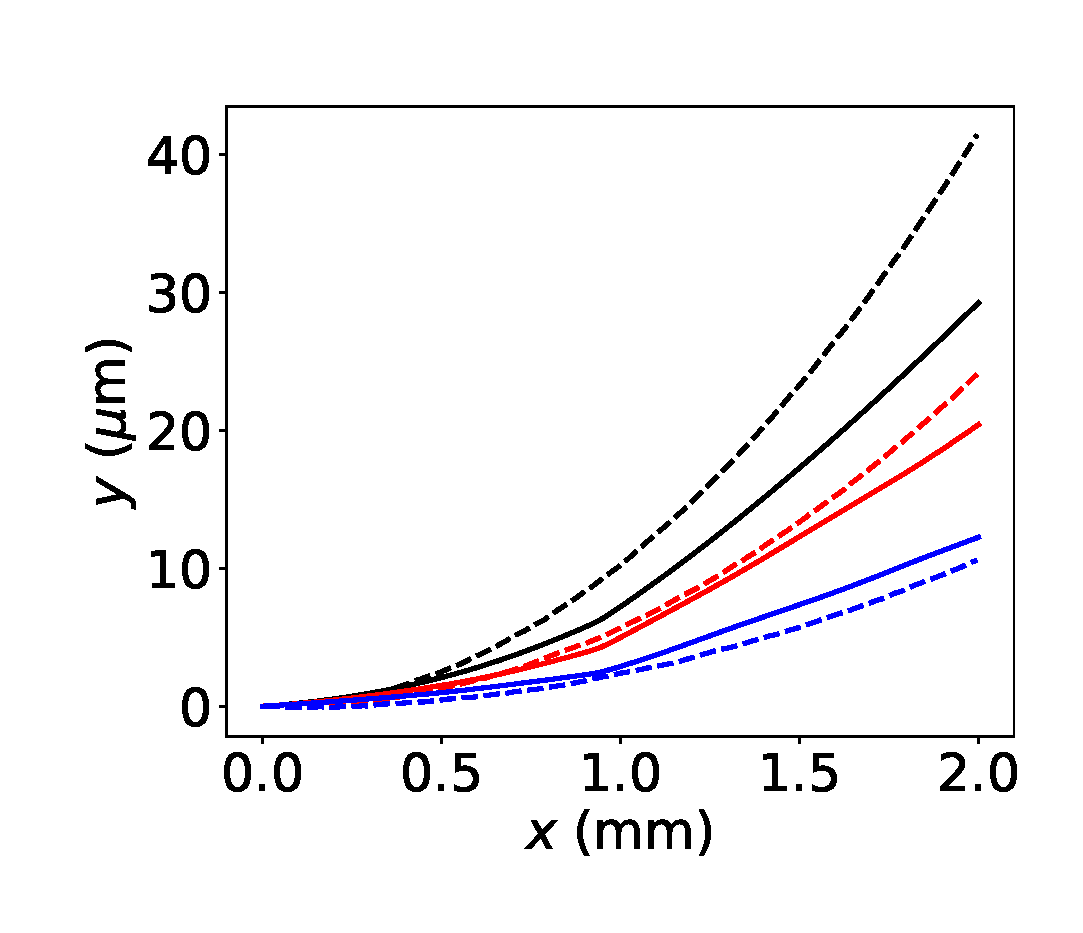
\includegraphics[scale=0.32]{rayparaxH100.eps}&
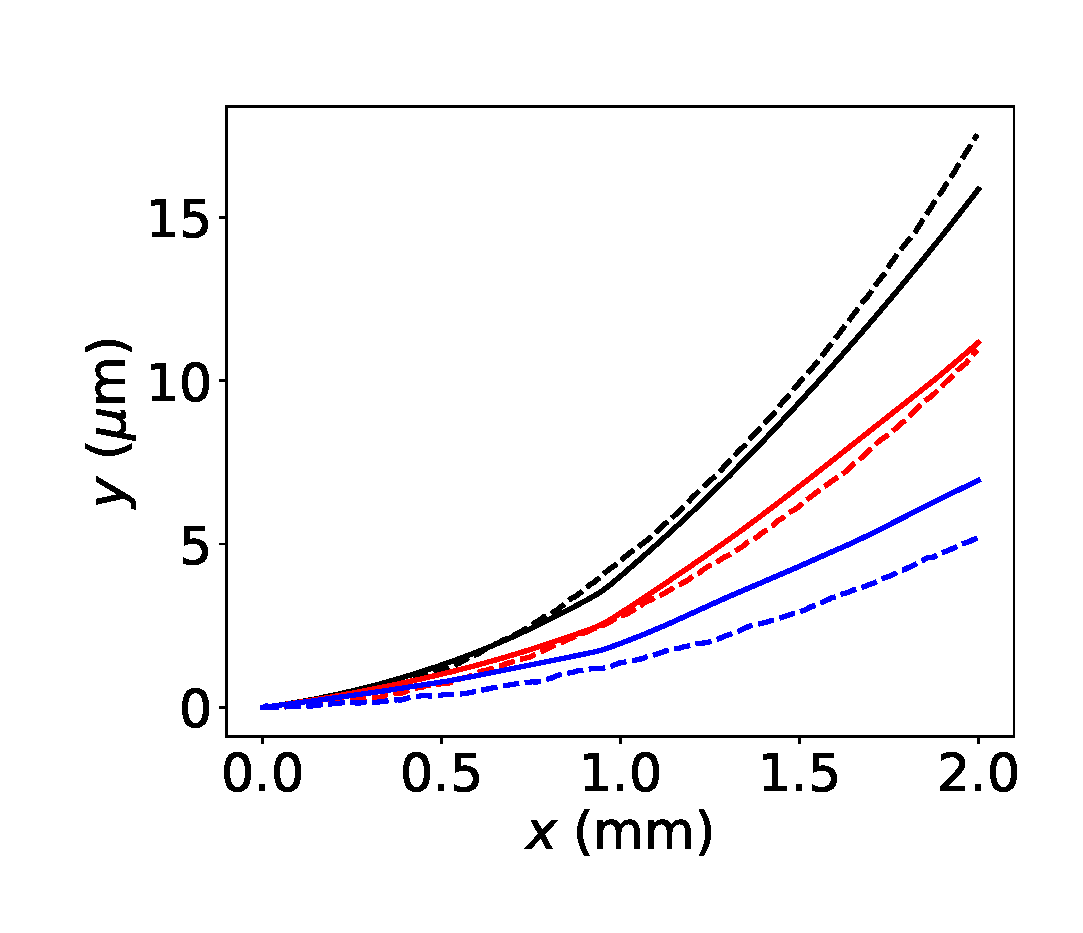
\includegraphics[scale=0.32]{rayparaxHe.eps}
\end{tabular}
\caption{ \label{fig:ssd} 
(a,b,c) Beam centroid, defined as $\Delta y =\int I(y)y dy/\int I(y) dy$, at $x=2\,\rm mm$ of the intensity profile resulting from HERA paraxial simulations (plain lines) for spectral dispersion mode numbers (defined at three $\omega$)
$\Delta =9$ (black), $15$ (red) and $33$ (blue). The temporal averaged of HERA centroids between $20$ and $90\,\rm ps$ correspond to the circles. 
The predictions of Eq. \eqref{eq:bbssd} are superimposed as dashed lines for $S=1$.
(d,e,f) Laser centroid as a function $x$ from the modified ray tracing scheme implemented in HERA (dahsed lines, Eq. \eqref{eq:raybb} with $S=1$) and from the HERA paraxial simulations as plain lines. The paraxial results are averaged between $20$ and $90\,\rm ps$ and the colors code for the same spectral dispersion strengths than panels (a,b,c).
}
\end{figure*}
As the pulse deflection is reduced by its loss of temporal coherence,  large simulation domains have to be considered in order obtain clean quantitative comparisons.
We thus aim  at building and validating a realistic pulse speckle scale beam bending model   in light of 2D HERA hydrodynamic simulations \cite[]{Loiseau_2006} [combining Eqs. \eqref{eq:beta2}, \eqref{eq:drakeh} and \eqref{eq:bbf}], therefore excluding kinetic effects such in multi-ion species plasmas or moderate $Z_iT_e/T_i$-values. In Sec. \ref{sec:icf} however, use will be made of the kinetic deflection rates.

As the value of the acoustic wave damping rate, $\nu$,  is critical for quantitatively capture the beam bending physics, we used in our HERA simulations a damping acoustic term (here noted $D$) acting on the component of the conservation of momentum  transverse to the laser direction: 
\begin{align}
(\partial_t + \mathbf{v}_d\cdot \nabla_\perp) \mathbf{v}_\perp + D  = - c_s^2\nabla_\perp\left(\frac{  \delta n }{n_0} +  \Phi  \right) \, ,\label{eq:hydro2} \\
D=  \mathrm{FT}^{-1}\left[ 2 c_s  \gamma_0 \vert k \vert   \hat{\mathbf{v}}_\perp  \mathrm{H}( k_0 - \vert k \vert )\right]\, ,
\end{align}
where $\mathrm{H}$ is the step function. Similar damping terms are used in other hydrodynamic codes \cite{phd-PEML,Masson_2006,Huller_2008} and ensure, despite expensive kinetic simulation results,  an accurate modeling of the acoustic wave propagation. 
In order to reach more realistic ICF-conditions than in Ref. \cite[]{POP_Ruyer_2020}, the choice has been made to use a laser wavelength of $\lambda_0=0.35\, \rm\mu m$  and  an electron density of $n_e = 0.1n_c$.
A 2D domain of size  $L_x\times L_y = 2\, \rm{mm} \times 1.024 \, \rm{mm}$ with the left boundary condition located at $x_\mathrm{BC}=0$ will be used. 
A RPP and SSD beam  or a ray tracing beam propagating in the $x$ direction were injected from the left boundary.
The focal spot is located at the center of the simulation domain, $x_\mathrm{foc}=1\, \rm mm$ with a focal number of $f_\sharp = 6.5$, a temporal
and spatial envelope following
\begin{align}
    \hat{g}(y) &= \exp(-\vert y\vert ^o/2\sigma_g^o)  \,  \label{eq:g}\\
    h(t) &= \mathrm{min}(t/\tau_h,1) \,\label{eq:h}
\end{align}
with $\tau_h=1\, \rm ps$,  $o=5$ and $\sigma_g = 300\,\rm \mu m$. 
For sake of simplicity and comparison purposes, the bremsstrahlung energy deposition is neglected in HERA-ray and HERA-parax and the non-local thermal correction of Eq. \eqref{eq:nl} is ignored in this section.  
Moreover a barotropic gas is assumed in the hydrodynamics simulations.  An electron density of $n_e =0.1n_c $ is used  and a $y$-aligned drift velocity, $v_y=v_d$, is imposed on both the electron and ion populations.
The  spectral dispersion  has a modulation frequency of  $\omega_m = 14.25\,\rm GHz$ and a mode number of alternatively $
\Delta = 9$, $15$ and $33$ (defined at $2\pi/k_0=0.35\,\rm\mu m$) corresponding to a speckle coherence time of 
$\tau_\mathrm{SSD} =2\pi/\omega_m/(2\Delta+1) =3.69$, $2.26$ and  $1.04 \,\rm ps$ respectively. 
The paraxial simulations mesh sizes follow $dx = 0.32\, \rm \mu m$ and $dy =0.0625\, \rm \mu m$. 
%Our paraxial, gathered in Fig. \ref{fig:ssd}, evidence a strong deformation of the beam spatial envelop for low SSD mode numbers [Fig. \ref{fig:ssd}(a)]. When $\Delta$ increases to $15$ (b) or $33$ (c), less warping and a more symmetric intensity profile is    obtained, indicating that less speckle-scale beam bending occurs.
%Figure \re{fig:} evidence a temporal oscillation of the beam centroid at the simulation exit plane, around a finite value. Indeed, 

Due to the phase modulation, the beam's center oscillates as soon as its injection and  on a period given by the modulation frequency, $2\pi/\omega_m\simeq 70\,\rm ps$. This leads to the centroid periodic movement at the simulation exit plane as shown as  plain lines in Figs.  \ref{fig:ssd}(a,b,c). The SSD ray tracing scheme that we will introduce aims at predicting the temporal averaged of the beam centroid deflection only, illustrated for the paraxial results as circles in Figs. \ref{fig:ssd}(a,b,c), therefore neglecting the spatial envelope's motion.
Assuming the hot spots to be independent and of Gaussian form, we may relate the time-averaged beam centroid deflection rate to the  contribution of the speckles ($s$-subscript) through, 
\begin{align}
  \frac{d\theta_\mathrm{SSD}}{dx}  =   \langle \sum_s\frac{d\theta_s}{dx}\rangle_t \, ,
  \end{align}
  where   $\langle x\rangle_t$ is the averaged of $x$ over a $2\pi/\omega_m$ period.
We will now, while using  Eq. \eqref{eq:bbf}, replace $\sigma$ by $\sigma\sqrt{1+(x-x_s)^2/z_c^2}$ and $I_0$ by $I_s/[1+(x-x_s)^2/z_c^2]^{1/2}$, where $x_s$ and $I_s$ are the speckle centre  and intensity respectively and where $z_c=\pi f_\sharp^2\lambda_0$, leading to 
  \begin{align}
 \frac{d\theta_\mathrm{SSD}}{dx}  &=   -S f_\mathrm{SSD} A_k \frac{n_0 }{n_c}  \frac{  I_0 }{ 4 v_g n_c T_e } \sqrt{\frac{2}{\pi}}   \frac{\beta_\mathrm{k/f}^{(D)} }{ \sigma}      \, , \nonumber \\
 S &=\sum_s \frac{I_s/I_0}{1+\frac{(x-x_s)^2}{z_c^2}}  \, , \nonumber \\
  f_\mathrm{SSD}  &= \langle f(t) \rangle_t = \int_0^{\mathrm{min}(t,\tau_\mathrm{SSD})} f(t) \frac{dt}{\mathrm{min}(t,\tau_\mathrm{SSD})} \, . \label{eq:bbssd}
  \end{align}
Hence, $ f_\mathrm{SSD}$ is a scalar that mainly depends on the local value of $\nu\tau_\mathrm{SSD}$, and which simplest form may be obtained by approximating $f(t)\simeq 1-e^{-\nu t}$ (thus neglecting the acoustic beamlets)  so that, in the following, use will be made of 
\begin{equation}
     f_\mathrm{SSD} \simeq \frac{\nu\tau_\mathrm{SSD}+ e^{-\nu\tau_\mathrm{SSD}} -1}{\nu\tau_\mathrm{SSD}}\, . \label{eq:fssdf}
\end{equation}
The factor $S$ in Eq. \eqref{eq:bbssd}, which encloses the impact of the speckle dynamics on the beam deviation, will in the following, be assimilated to a scalar thus smoothing out the hot spot contributions over the whole pulse.  This final approximation implies to neglect the speckle scattering disparities resulting from the variability of their intensity (see Sec. \ref{sec:speckle}).
Our 2D paraxial hydrodynamic simulations suggest that $S\simeq 1$, as used in the following, and  lead to satisfactorily agreement between the theoretical predicitons [dashed lines in Figs. \ref{fig:ssd}(a,b,c)] and the temporally averaged paraxial results (as circles). Note that the  value of $S$ could  change in three dimensional systems. 
%
%Figures \ref{fig:ssd}(a,b,c) illustrates for three different plasma parameters, the dependence on time of the laser centroid after two millimeters for propagation as predicted by the paraxial HERA simulations and for different spectral dispersion strength. After $\sim 10\,\rm ps$, an oscillation of $\Delta y$ of period $2\pi /\omega_m = 90\,\rm ps$ around an asymptotic limit is evidenced. This oscillations,  observable in vacuum, are due to the motion of the laser centroid caused by the spectral dispersion and is completely ignored from most crude modeling such as ray tracing schemes. A temporal averaged between $t=20\,\rm ps$ and $20+2\pi/\omega_m\simeq 70\,\rm ps$ will thus be applied to our paraxial results [as circles in Fig. \ref{fig:ssd}(a,b,c)] for our predictions. 
Finally and as expected, the increase of the  mode number ($\Delta$) decreases the beam deviation and is well captured by our model. 

\subsection{Accounting for beam bending with spectral dispersion in  ray tracing schemes}\label{sec:ray}
In this context, the time-averaged centroid deviation rate  may naturally be implemented in a ray tracing scheme as a correction to the well-known refraction deviation rate, by deflecting each ray accordingly to   Eq. \eqref{eq:bbssd}.
The ray directions and positions ($\mathbf{k}$ and  $\mathbf{r}$ respectively)  therefore verify
\begin{align}
    \frac{d\mathbf{k}}{ds} &=-k_0 \frac{\nabla n_e }{2n_c\eta} -k_0\frac{n_0 }{n_c}  \frac{  S f_\mathrm{SSD} A_kI_0 }{ 4 v_g n_c T_e } \sqrt{\frac{2}{\pi}} \frac{\beta_\mathrm{k/f}^{(D)} }{ \sigma}  \frac{\mathbf{v}_\perp}{\vert \mathbf{v}_\perp \vert }\, \nonumber\\
        \frac{d\mathbf{r}}{ds} &= \frac{\mathbf{k}v_g}{\omega_0} \, , \nonumber\\
    \mathbf{v}_\perp&= \mathbf{v}_d - \frac{ \mathbf{v}_d\cdot \mathbf{k}}{\vert  \mathbf{k}\vert^2}\mathbf{k}\, \label{eq:raybb}
\end{align}
where $s$ is the ray abscissa and $\eta$, the optic index.

The above model has been implemented in a new  ray  tracing module of the hydrodynamical code HERA \cite[]{Loiseau_2006}.
For solving the ray trajectory, we split the rectangular meshes in four triangles using their diagonals.  In each triangle, the density profile is assumed to be planar allowing to have a continuous density profile in all the simulation domain. 
Hence, solving the Eikonal equation  in each triangle allows to break the ray trajectory in a row of parabolas ideal for fast computing. 
Summing the contribution of each rays that pass through a given mesh following Ref. \cite[]{POP_Debayle_2019}, one obtains the local averaged intensity, $ I_0$, used in Eq. \eqref{eq:raybb}.
So has to mimic the averaged intensity profile at and off best focus, we define a lens position, hereafter at $x_\mathrm{lens}=-10$ m from which rays are shot. 
The rays departure $y$-positions  on the lens are chosen randomly, and their initial direction points toward a randomly distributed  position at the focal plane (at $x=x_\mathrm{foc}$) which ascertain the power carried by the ray so as to fulfill the required intensity profile at best focus [given by $g(y)$]. 
Finally, the rays are propagated  in vacuum from the lens to the left boundary condition  of the simulation (at $x=x_\mathrm{BC}$).
In order to avoid statistical bias, the position and directions of the rays are shot at beginning of each time steps. 
Note that this procedure locally gives a  finite   transverse opening angle to the ray distribution, thus avoiding unphysical thermal filamentation  arising from perfectly parallel as used in Refs. \cite[]{Colaitis_2014,Lefebvre_2018}.
Finally, a mesh size of    \textcolor{red}{   $dx = 10\, \rm \mu m$ and $dy =10\, \rm \mu m$} is used along with  $10^4$ rays. All other simulations characteristics (equation of states, boundary condition and simulation domain) are identical to the paraxial simulations, as described in \ref{sec:parax}.

Until now, we assumed  $\mathbf{v}_d$ to be perpendicular to the main laser axis, which is wrong most of the time in a realistic system. Hence, the axis on which the beam bending contribution in Eq. \eqref{eq:raybb}  lies results from the projection,  $\mathbf{v}_\perp$, of the fluid velocity $\mathbf{v}_d$ on the plane perpendicular to the ray direction, $ \mathbf{k}$.
Importantly, this modification to the classical ray tracing scheme [Eq. \eqref{eq:raybb}] remains minimal as it does not modify the  ray propagation main algorithm (described above) apart from adding a dependence on the beam intensity of the ray deflection rate. 
Overall, the centroid deviations resulting from the modified ray tracing module of HERA as dashed lines in Figs. \ref{fig:ssd}(c,d,e) reproduce correctly the temporally averaged paraxial predictions (plain lines) as predicted for the three plasma parameters and three SSD-strength considered.

It is important to note that restricting the model to the  beam centroid deviation implies to neglect the  different deflections caused by  the various speckle intensities  and lifetimes,  contributing to the beam spreading as discussed in Sec. \ref{sec:speckle}. Likewise, the forward Brillouin instability \cite[]{POP_Grech_2006,PRL_Grech_2009,phd-Grech} and associated plasma smoothing effects may contribute to enlarge the beam waist, modify the speckle distribution and affect the centroid deviation. 
Moreover, our crude modeling of the speckle dynamics does not  account for the oscillations of the coherence time and speckle velocity  as characterized in Ref. \cite[]{POP_Cain_Riazuelo_2012}, which also contributes to the fluctuation  of the beam direction. 

\section{Quantifying the beam bending of a  realistic pulse in  ICF conditions}\label{sec:icf}
\begin{figure*}
\begin{tabular}{ccc}
(a)Total laser power & (b) $\langle Z_i\rangle $& (c) $\langle Z_i\rangle T_e/T_i$
\\
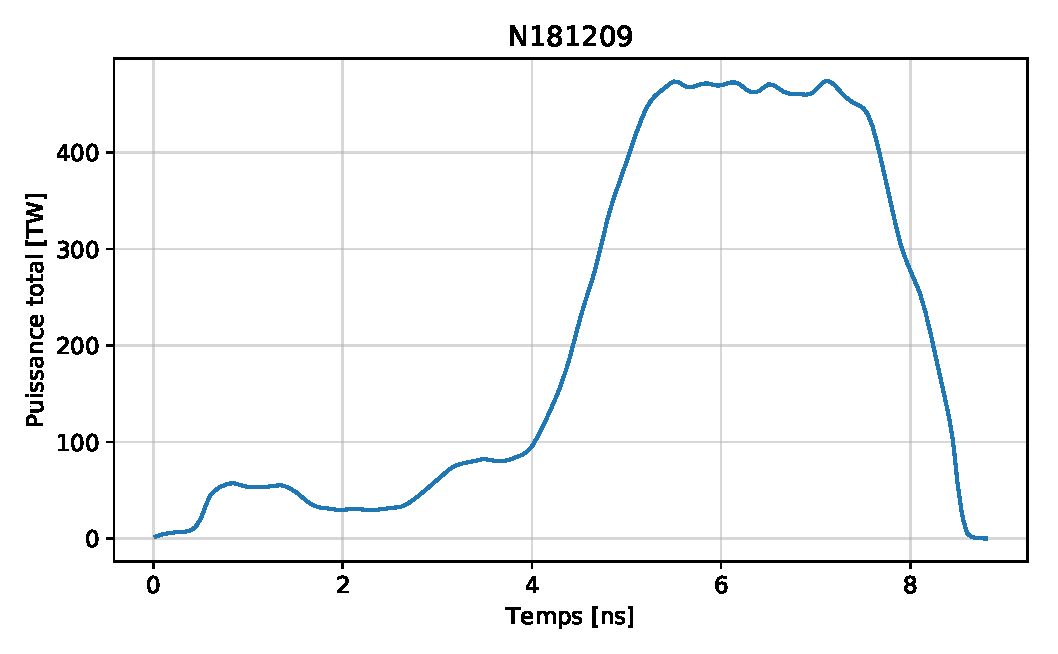
\includegraphics[width=0.25\textwidth]{Plasertotale.pdf}&
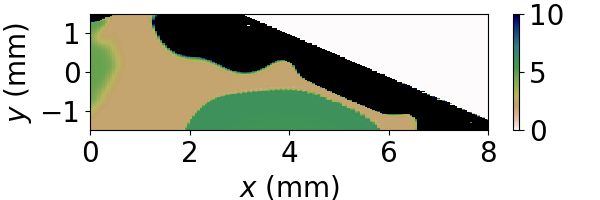
\includegraphics[width=0.33\textwidth]{Z5ps.png}
&
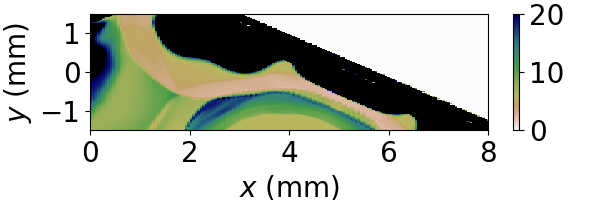
\includegraphics[width=0.33\textwidth]{ZTesTi5ps.png}\\
(d)  $f_\mathrm{SSD}$   &
(e) $n_e/n_c$
&(f) $d\theta_\mathrm{SSD}/dx$ ($^o/$mm) \\
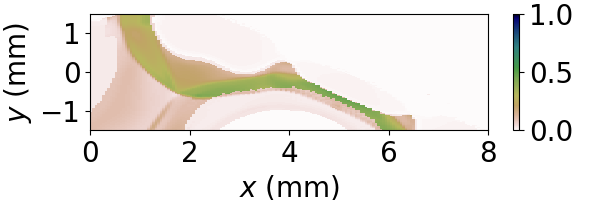
\includegraphics[width=0.33\textwidth]{f5ps.png} 
&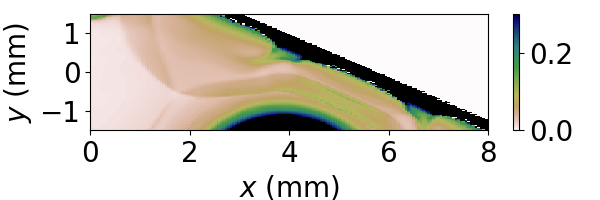
\includegraphics[width=0.33\textwidth]{ne5ps.png} 
&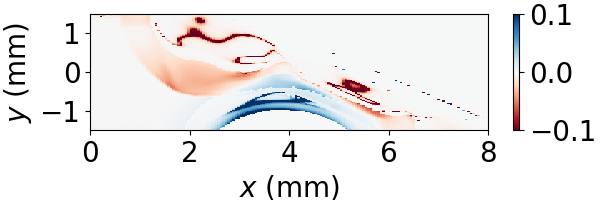
\includegraphics[width=0.33\textwidth]{dtheta5ps.png}\\
(g) $\log(I\, [\mathrm{W/cm^2}])$, rays with bending &(h)  $\log(I\, [\mathrm{W/cm^2}])$, rays without bending&(i) Lineout along the gold wall\\
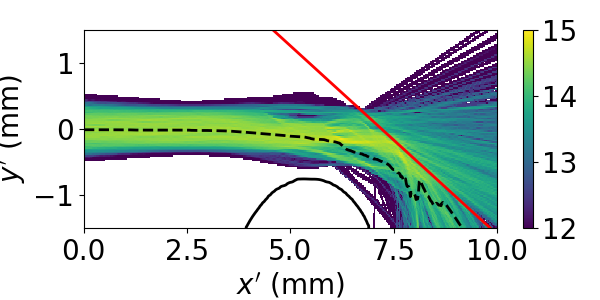
\includegraphics[width=0.33\textwidth]{raybb_FCI2.png} 
&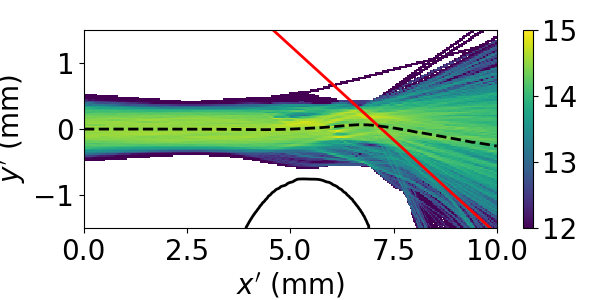
\includegraphics[width=0.33\textwidth]{raybb_FCI2_nobb.png} 
&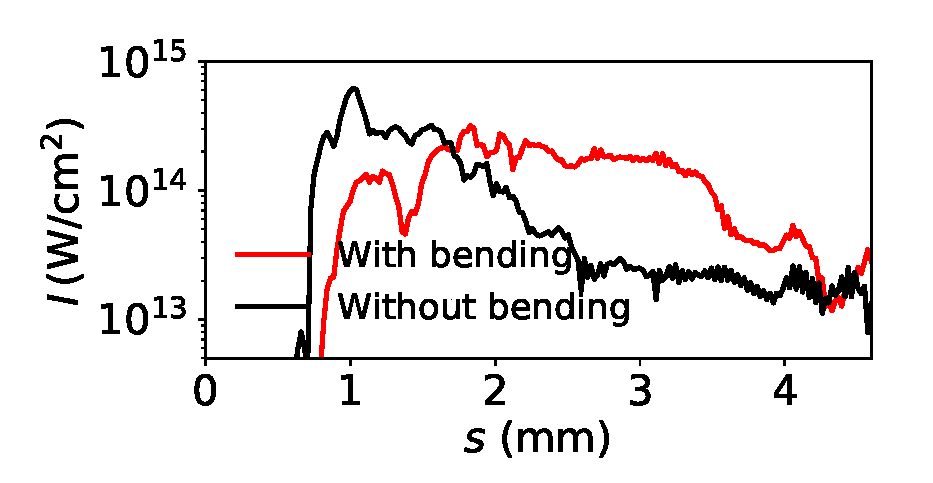
\includegraphics[width=0.33\textwidth]{raybb_FCI2_lineout.eps}
\end{tabular}
\caption{ \label{fig:icf} 
Hydrodynamic simulation performed with the code FCI2 of a $1.8$ MJ NIF shot for a diamond ablator imploding capsule in a gold hohlraume with low pressure gaz fill and illustrated in the frame of the inner cone ($y=0$ is the main inner cone axis). 
(a) Total power of the main laser drive.
 Averaged local ionisation number, $\langle Z_i\rangle$ (b), $\langle Z_i\rangle T_e/T_i$-ratio (c),
transient function of Eq. \eqref{eq:fssdf} computed on the local plasma parameters for a speckle coherence time $\tau_\mathrm{SSD}=6\,\mathrm{ps}$ (d) and normalized electron density (e).
(f) Two dimensional  deflection rate as predicted by Eqs. \eqref{eq:beta2}, \eqref{eq:drakek} and \eqref{eq:bbssd} calculated for    $I_0=3.2\times 10^{14}\,\mathrm{W/cm^2}$.
(g,h) Intensity profile in log scale as predicted by the modified  (g) and classical (h) ray tracing scheme, Eq. \eqref{eq:raybb}. The ablator and gold wall positions are superimposed as black and red plain lines respectively.   The beam centroid defined as $\int I(y)y dy/\int I(y) dy$ is illustrated as black dashed lines. 
(i) Intensity lineout along the red plain line in (g,h).
Panels (b-i) correspond to  $t=5\,\rm ps$.
%The limits of the inner and outer cone are superimposed on panel (a-c,e) as black dashed and plain lines respectively. 
}
\end{figure*}
In order to quantify the beam bending level in realistic conditions, we performed a FCI2 hydrodynamic simulation of a diamond  ablator capsule implosion in a  low gaz-fill hohlraume \cite[]{Lefebvre_2018}.
One  representative  time was retained,  $5\,\rm ns$, which corresponds  to  the end of the rise of the main drive, as illustrated in Fig. \ref{fig:icf}(a).
We will here focus on the beam bending of the inner cone, which main axis lies in $y=0$ and propagates  from left to right in  Figs. \ref{fig:icf}(b-f). 
The beam bending deflection rate is   calculated using the local plasma parameters with the averaged intensity $I_0=3.2\times 10^{14}\,\rm W/cm^2$ and a speckle coherence time of $\tau_\mathrm{SSD}=6\,\rm ps$ using the 2D kinetic formalism  of Eqs.  \eqref{eq:beta2}, \eqref{eq:drakek} and  \eqref{eq:bbssd}, accounting for the non local correction of Eq. \eqref{eq:nl}.

Figures \ref{fig:icf}(a-f), correspond to the local $\langle Z_i\rangle$, $\langle Z_i\rangle T_e/T_i$, $f_\mathrm{SSD}$ and demonstrate that, at $5\, \rm ns$, moderate values of $\langle Z_i\rangle T_e/T_i\le 5$ may be found on the inner beam path, suggesting significant kinetic contributions [see Fig. 3 of Ref. \cite{POP_Ruyer_2020}]. Indeed, as the helium gas is being compressed by the expending  ablator [green region in Fig. \ref{fig:icf}(b)] and gold wall [black region in Fig. \ref{fig:icf}(b)], the ion temperature significantly increases and the electron density remains in the $10\%$ critical density range. Likewise, the electron temperature, in excess of $2$ keV in these regions (not shown), leads to qualitatively small Landau damping rates and  therefore $f_\mathrm{SSD}$-values close to unity [see Fig. \ref{fig:ssd}(d)]. 
The temporal incoherence is thus not strong enough to significantly alleviate the beam bending, leading to significant deviation rates, as illustrated in Fig. \ref{fig:ssd}(f) in the gaz region and in the carbon ablator. 
%
%A deflection rate of $0.1\,\rm ^o/mm$ extending on $2$ mm and a fraction of $0.05\,\rm ^o/mm$ on $2-3$ mm at $3.5$ and $5\, \rm ps $ respectively is therefore predicted which should, once projected on the gold wall  $\sim 3\, \rm mm$  away, should end up in an averaged deviation of $\sim 200\,\rm \mu m$. Additionally, unlike in our academic paraxial simulations, the  beam deviation, far from being homogeneous, is of opposite polarity  at $x\simeq 2$ and $4\, \rm mm$ which should significantly affect the beam pointing, once projected on the gold wall. 
Note that, at $5\,\rm  ns$, the density of the expended window is of the order of $n_e\sim 10^{-3}n_c$  [see Fig. \ref{fig:icf}(e)]  which is too small for the speckle scale beam bending to occur.

Two ray tracing HERA simulations have been performed using the plasma profiles resulting from FCI2  [Figs. \ref{fig:icf}(b-f)] while truncating the high density part at $n_e=0.2n_c$, the first  models the inner cone with the modified scheme of Eq. \eqref{eq:raybb} (g) and the second, with the  classical ray propagation (h). 
Apart from a larger domain size of $L_x\times L_y = 8 \times 3 \, \rm mm^2$ and the plasma profiles, all other parameters are identical to the ray tracing simulations described in   Sec. \ref{sec:ray}.  The resulting intensity profiles illustrated in Figs. \ref{fig:icf}(g,h) evidence a drastic impact of the beam bending dynamics on the pointing direction.  When accounting for the beam deviation (g), the region located around $x=2\,\rm mm$ tends to deflect significantly the laser toward the ablator (as black plain line) where  both the beam bending rates and the refraction due to the density gradients are important. As a result, a significant part of the laser energy is deviated and does not seem to reach the gold critical surface [as a red plain line, located in the region $\langle Z \rangle>10$ in Fig. \ref{fig:icf}(b) and $n_e\ge 0.2n_c$ in (e)]. Finally, the gaz motion which is downward around $x=2\,\rm mm$ due to the gold expansion and upward at $x=4\,\rm mm$ because of the ablator, along with the refraction of light ends up, not only in a beam centroid deviation but also to a significant beam spreading as illustrated by the lineouts of the laser intensity profile along the gold wall [see  Fig. \ref{fig:icf}(i)].
Hence, the comparison of Figs. \ref{fig:icf}(g) and (h)  demonstrates that a sensible part of the inner cone is deflected, due to the speckle scale  beam bending, toward the hohlraume main axis and never reaches the high  density and laser-absorbing part of the expending gold. 
Indeed, the deflection rate in Fig. \ref{fig:icf}(f) of  $\sim \pm 0.05\,\rm ^o/mm$ extending over  $2-3$ millimeters  (which corresponds to a modest averaged deviation of $\sim 200\,\rm \mu m$ once projected on the gold wall), is enough at grazing incidence to significantly modify the beam's refraction.
As a result, a large difference between the intensity lineouts at the gold wall [red plain line in Figs. \ref{fig:icf}(g,h)] is characterized in Fig. \ref{fig:icf}(i), leading to a much broader profile  and a  centroid shift of roughly one millimeter when accounting for the beam bending physics.
The deflected beam path could lead to the opposite laser entrance hall 
and therefore to a possible wave mixing with opposite-side beams. A striking qualitative similarity with experimental measurements ascribed to stimulated Brillouin side scatter or the so-called glint \cite[]{Honda_1998,PRL_Turnbull_2015}  urges to address the possible interweaving of beam bending with these processes and the impact   on  the implosion symmetry in ICF experiments.

Some  of our paraxial HERA simulations indicate, in addition to the centroid deviation, a contribution to the beam spreading   due to the stimulated forward Brillouin scattering \cite[]{PRL_Grech_2009,POP_Hinkel_1998}. 
Since our study is limited to the beam centroid deviation, further analysis, including forward scatter and beam spreading, are required in order to properly understand all the physical mechanism able to affect the beam pointing and subsequent laser energy deposition region inside the hohlraume.
Additionally, ray tracing model with spectral dispersion has been compared to   homogeneous ideal simulations, so that, its   validity should be ensured in   smooth density gradients only. Significant geometrical effects are also to be expected, however,  the three dimensional paraxial simulations required to fit our ray tracing scheme in realistic geometry are out of the scope of this manuscript as we settled with a 2D analysis.
In the region of large bending rate [$1\,\mathrm{mm} \le x\le 4\,\mathrm{mm}$ in Fig. \ref{fig:icf}(f)], Fig. \ref{fig:2d3dnl} indicates that  the two dimensional geometry overestimates the  3D counterpart by a factor $\sim 2$ at resonance, thus suggesting  an overestimation of the flow  deflection in Figs. \ref{fig:icf}(g-i). 
Nevertheless, the significant differences evidenced in Fig. \ref{fig:icf}(i) incites us to address the impact of the beam bending physics on the irradiation geometry in three dimensional ICF conditions.

\section{Conclusions and prospects}
Based on a previous publication, we addressed the beam bending physics of RPP and SSD high-energy laser pulse propagating in  ICF-like plasma conditions. 
By mean of large homogeneous paraxial hydrodynamic simulations, we constructed a 2D ray-tracing model which  quantitatively capture the temporally averaged  centroid deviation  of spatially smoothed pulse  with moderate to large spectral dispersion. The limit of our model appears when  plasma smoothing effects are able to affect significantly the speckle distribution, of importance for small SSD mode numbers or for RPP beams. 
However, the use of our ray tracing model in realistic conditions demonstrates that significant modifications of the beam propagation properties, possibly affecting the implosion dynamics, results from the speckle scale beam bending in realistic pulses. 
Hence, the speckle-scale physics  may be included in coarse description of light such as  ray tracing-based schemes, opening the way for a more realistic laser energy deposition in radiative hydrodynamic codes and possibly a more accurate prediction of the implosion symmetry. 

Note that, although not presented in this paper, adapting the present model to  three dimensions seems straightforward as the 3D kinetic  beam bending rates have been derived and that the modified ray-tracing scheme, as presented in this study, remains valid in realistic geometry. This may require to run three dimensional paraxial simulations  of a realistic pulse propagation as the fitted parameter  of Eq. \eqref{eq:dthssd}  probably depends on the system geometry.  
The 3D effects  could somewhat alleviate  the large impact of the beam bending physics on the laser propagation evidenced in this study.
Additionally, the deviation in multi-ion species plasmas present important kinetic contributions and the corresponding transient regime remain unexplored. 
In these plasmas,  our ray tracing model fails to be predictive and a dedicated kinetic study is required.
Moreover, most wave-mixing processes are absent from our analysis, possibly affecting the beam deflection and bringing further complexity to the system \cite[]{POP_Huller_2020}.

\section*{Acknowledgements}
We acknowledge fruitful discussions with S. Laffite.
 \textcolor{red}{We also acknowledge D. Dureau and the HERA-team for all their work on the HERA code. }
This work has been done under  the auspices of  CEA-DAM and
the simulations were performed using HPC resources at TGCC/CCRT and CEA-DAM/TERA.
\bibliography{biblio}
\end{document}
